The \class{LocalSearchEngine} class uses the model created for local search described in section \ref{sec_ls} and 
uses local search to improve the initial solution. The vector holding pointers to the independent variables is given a 
random ordering, called a mask, that is used in local search. \\
Local search explores how changing the value of few variables will affect the solution quality, hence exploring a 
neighbor 
solution. The key for being efficient is to compute this change fast. The dependency digraph and the propagation 
queues are used for this. Before committing a neighborhood operation several neighborhood operations might be explored 
before choosing one to commit. To evaluate a neighborhood operation a delta value for each invariant is used. The 
delta value is the value an invariant would change if the neighborhood operation is committed. By this we can evaluate 
the neighbor solution without committing a neighborhood operation. \\
Each constraint $c \in C$ created in the model was given a priority $p$ and these priorities are used during local 
search. Let $k$ denote the highest priority given. A new \class{Sum} invariant is created for each priority $p$ and 
one for the objective function. This is done at the same time invariants are created by each constraint class. \\
Let $q_p \in Q$ be the sum of violation degree of the constraints with priority $p$. The objective functions 
value is consider as $q_0$ and the vector $Q$ is used to evaluate the quality of a solution. The evaluation function 
$f(\tau)$ is not returning a single value but the quality vector, $f(\tau) = Q_\tau$.  \\ 
Two candidate solutions $\tau$ and $\tau'$ each have a vector of quality $Q_\tau$ and $Q_{\tau'}$ respectively. To 
determine which of the two solution are best their vector can be compared, starting with position $k$ and going 
backwards. The first time they differ in value determine which solution is best, the one with the lowest value. 
Illustrated with a small example:
\begin{align}
 Q_\tau &= (5,2,4,2) \\ 
 Q_{\tau'} &=(10,6,3,2) 
\end{align}
Violation degrees of constraints with priority 3 ($Q_\tau[3]$, $Q_{\tau'}[3]$) contributes with 2 in each candidate 
solution and then the violation degree of constraints with priority 2 is consider. Then candidate solution $\tau'$ is 
consider better than $\tau$ since $Q_\tau(2) = 4$ $>$ $Q_{\tau'}(2) = 3$. \\
The new classes used for local search are in three different categorize; moves, neighborhoods, and search 
procedures. A \class{Move} object stores information of a neighborhood operation including the change of the evaluate 
function. A subclass of the \class{Neighborhood} class is the choice of neighborhood function and gives the 
sequence in which the neighbor solutions in the neighborhood graph are explored. The search procedures can query a 
\class{Neighborhood} class to evaluate a neighborhood operations, a \class{Move} class, effect on the evaluation 
function. The search procedures determine which neighborhood operation to commit, if any. Neighborhoods and 
search 
procedures are combined to create different local search algorithms and \class{LocalSearchEngine} uses them within the 
time limit to search for a better solution. \\
The first algorithms that is used is a first improvement until a local optmia is found. Gecode is not used to optmize 
hence it might be posible to improve the initial solution very easily. If Gecode does not find an initial solution it 
is very likely that the construction heuristic, random assignment, does not give a feasible solution and is far from a 
local optima. It is prefered to start in local optima or at least close to one and first improvement is very efficient 
at finding a local optima. \\
\begin{figure}[!t]
\begin{center}
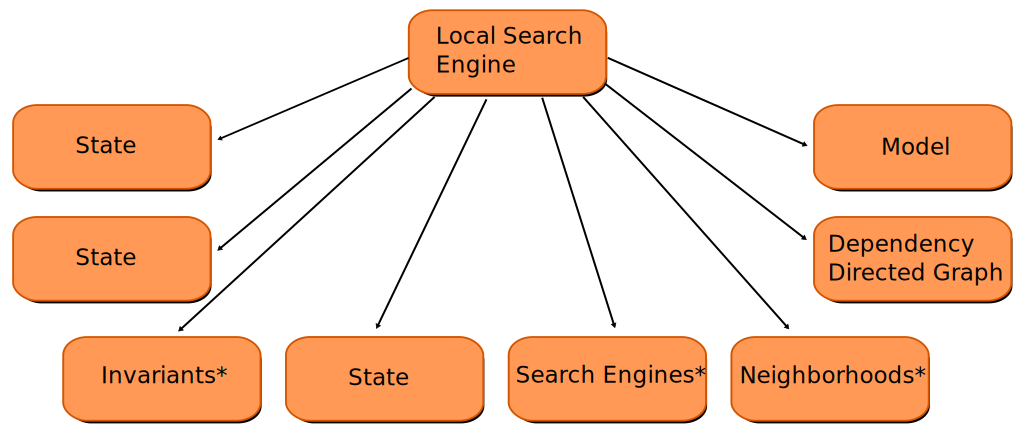
\includegraphics[width=0.9\linewidth]{LSE}\caption{Overview of the class pointers of \class{LocalSearchEngine}. The 
fields marked with a star (*) are several classes of that type.} 
\label{fig_lse}
\end{center}
\end{figure}\noindent




% For simplicity let us first consider the neighborhood operation involving changing the value 
% of a single 
% variable $x$. The change of variable value is send through the dependency digraph where each invariants, reachable from 
% the vertex representing $x$, is updated. The propagation queue is used to determine the sequence the invariants should 
% be updated. This will update invariants that represent violation of constraints with different priority and the 
% evaluation function. \\
% If a neighborhood operation consist of more variables changing values, such as swapping values of two variables, the 
% propagation queues 
% of these variables can be merged. The merging should remove duplicates and keep the invariants topological sorted. The 
% invariants unique time stamp can be used to keep the ordering. The new queue gives an ordering the invariants should be 
% updated such that they are only updated once during each neighborhood operation. \\ 